\def\mainpage{mainpage}

\ifx\mainpage\undefined
\documentclass[twoside, doctor, fontset=windows]{../misc/BIT-thesis-grd}
%跨文件引用
\usepackage{xr}
%字体warning
\usepackage{anyfontsize}
\usepackage{float}
\usepackage{amsmath}
\usepackage{mathtools,nccmath}
\usepackage{amssymb}
\usepackage{latexsym}
\usepackage{wasysym}
\usepackage{graphicx}
\usepackage{subfigure} %图片插入
\usepackage{url}
\usepackage{algorithm}
\usepackage{algorithmic}
\usepackage{color}
\usepackage{tikz} %绘图
\usepackage{multirow}
% \usepackage{makecell}
\usepackage{bm}
% \usepackage{tabu}
\usepackage{booktabs}
\usepackage{verbatim}
\usepackage{geometry}
\usepackage{lettrine}
\usepackage{hyperref}
\usepackage{cleveref}
\usepackage[justification=centering]{caption}
\usepackage[acronym]{glossaries}

%各个章节标题
\newcommand{\maintitle}{老天也会宠幸笨小孩}
\newcommand{\englishmaintitle}{God Loves Fools, too}
\newcommand{\chptitleOne}{绪论}
\newcommand{\chptitleTwo}{老天的万分之一也会宠幸到我们这些笨小孩}
\newcommand{\engchptitleTwo}{One millionth part of God's gift would also come to us stupid kids}

%自定义符号
\renewcommand{\algorithmicrequire}{\textbf{输入:}}
\renewcommand{\algorithmicensure}{\textbf{输出:}}
\DeclareMathOperator*{\argmax}{arg\,max}
\DeclareMathOperator*{\argmin}{arg\,min}
\DeclareMathOperator*{\softmax}{softmax}


%独立符号
\newcommand\indep{\protect\mathpalette{\protect\independenT}{\perp}}
\def\independenT#1#2{\mathrel{\rlap{$#1#2$}\mkern2mu{#1#2}}}

\renewcommand\arraystretch{1.5}%表格行高
\AtBeginEnvironment{algorithmic}{\setstretch{1.36}}%算法行距

\crefformat{algorithm}{算法~#2#1#3~}
\crefformat{table}{表~#2#1#3~}
\crefformat{figure}{图~#2#1#3~}
\crefformat{equation}{公式~(#2#1#3)~}
\crefformat{footnote}{$^{#2#1#3}$}
\crefformat{chapter}{章节~#2#1#3~}
\floatname{algorithm}{算法}

\AtBeginDocument{
  \crefformat{section}{章节~#2#1#3~}
  \crefformat{subsection}{章节~#2#1#3~}
  \crefformat{subsubsection}{章节~#2#1#3~}
}

\definecolor{bitred}{RGB}{161,62,11}
\definecolor{bitgreen}{RGB}{0,164,68}
\newcommand{\myredbox}[1]{\tikz[baseline=(MeNode.base)]{\node[rounded corners, fill=bitred!20](MeNode){#1};}}
\newcommand{\mygreenbox}[1]{\tikz[baseline=(MeNode.base)]{\node[rounded corners, fill=bitgreen!20](MeNode){#1};}}


\else
\documentclass[twoside, doctor, fontset=windows]{./misc/BIT-thesis-grd}
%跨文件引用
\usepackage{xr}
%字体warning
\usepackage{anyfontsize}
\usepackage{float}
\usepackage{amsmath}
\usepackage{mathtools,nccmath}
\usepackage{amssymb}
\usepackage{latexsym}
\usepackage{wasysym}
\usepackage{graphicx}
\usepackage{subfigure} %图片插入
\usepackage{url}
\usepackage{algorithm}
\usepackage{algorithmic}
\usepackage{color}
\usepackage{tikz} %绘图
\usepackage{multirow}
% \usepackage{makecell}
\usepackage{bm}
% \usepackage{tabu}
\usepackage{booktabs}
\usepackage{verbatim}
\usepackage{geometry}
\usepackage{lettrine}
\usepackage{hyperref}
\usepackage{cleveref}
\usepackage[justification=centering]{caption}
\usepackage[acronym]{glossaries}

%各个章节标题
\newcommand{\maintitle}{老天也会宠幸笨小孩}
\newcommand{\englishmaintitle}{God Loves Fools, too}
\newcommand{\chptitleOne}{绪论}
\newcommand{\chptitleTwo}{老天的万分之一也会宠幸到我们这些笨小孩}
\newcommand{\engchptitleTwo}{One millionth part of God's gift would also come to us stupid kids}

%自定义符号
\renewcommand{\algorithmicrequire}{\textbf{输入:}}
\renewcommand{\algorithmicensure}{\textbf{输出:}}
\DeclareMathOperator*{\argmax}{arg\,max}
\DeclareMathOperator*{\argmin}{arg\,min}
\DeclareMathOperator*{\softmax}{softmax}


%独立符号
\newcommand\indep{\protect\mathpalette{\protect\independenT}{\perp}}
\def\independenT#1#2{\mathrel{\rlap{$#1#2$}\mkern2mu{#1#2}}}

\renewcommand\arraystretch{1.5}%表格行高
\AtBeginEnvironment{algorithmic}{\setstretch{1.36}}%算法行距

\crefformat{algorithm}{算法~#2#1#3~}
\crefformat{table}{表~#2#1#3~}
\crefformat{figure}{图~#2#1#3~}
\crefformat{equation}{公式~(#2#1#3)~}
\crefformat{footnote}{$^{#2#1#3}$}
\crefformat{chapter}{章节~#2#1#3~}
\floatname{algorithm}{算法}

\AtBeginDocument{
  \crefformat{section}{章节~#2#1#3~}
  \crefformat{subsection}{章节~#2#1#3~}
  \crefformat{subsubsection}{章节~#2#1#3~}
}

\definecolor{bitred}{RGB}{161,62,11}
\definecolor{bitgreen}{RGB}{0,164,68}
\newcommand{\myredbox}[1]{\tikz[baseline=(MeNode.base)]{\node[rounded corners, fill=bitred!20](MeNode){#1};}}
\newcommand{\mygreenbox}[1]{\tikz[baseline=(MeNode.base)]{\node[rounded corners, fill=bitgreen!20](MeNode){#1};}}


\fi


\ifdefined\chpabs
\externaldocument{../chapter1/chapter1}
\externaldocument{../chapter2/chapter2}
\fi

\ifdefined\chpOne
\externaldocument{../chapter2/chapter2}
\setcounter{chapter}{0}
\fi

\ifdefined\chpTwo
\externaldocument{../chapter1/chapter1}
\setcounter{chapter}{1}
\fi

\ifdefined\chpConcl
\externaldocument{../chapter1/chapter1}
\externaldocument{../chapter2/chapter2}
\fi


\ifx\mainpage\undefined

\newglossaryentry{YCY}
{
  name = {YCY},
  description = {杨超越(Yang Chaoyue,YCY)},
  first = {杨超越(Yang Chaoyue,YCY)},
  text = {~YCY~}
}



\begin{document}
\else

\newglossaryentry{YCY}
{
  name = {YCY},
  description = {杨超越(Yang Chaoyue,YCY)},
  first = {杨超越(Yang Chaoyue,YCY)},
  text = {~YCY~}
}



\graphicspath{{chapter1/}{chapter2/}{chapter3/}{chapter4/}{chapter5/}}
\fi


\begin{document}
%==============改数学字体设置,Latin Modern Math 默认的的确有点细,看个人需要,下面提供一种方法,需要的可以取消注释=========%
% \usepackage[bold-style=ISO]{unicode-math} %采用unicode-math,可以直接输入Unicode公式,当然传统的输入就行
% \setmathfont{XITS Math}  %目前unicode-math 支持几种数学字体,具体用法可以查看帮助文档,这里采用类似times字体科学数学字体,可以取消注释对比

%%%%%%%%%%%%%%%%%%%%%%%%%%%%%%
%% 封面
%%%%%%%%%%%%%%%%%%%%%%%%%%%%%%

% 中文封面内容(关注内容而不是表现形式)
\classification{TP000.0} 
\UDC{000.0} 

\title{\maintitle}
\vtitle{\maintitle}
\author{杨超越}
\institute{杨超越学院}
\advisor{杨超越}
\chairman{杨超越}
\degree{超越学博士}
\major{超越科学与技术}
\school{超越大学}
\defenddate{2020年6月}
%\studentnumber{**********}


% 英文封面内容(关注内容而不是表现形式)
\englishtitle{\englishmaintitle}
\englishauthor{Yang Chaoyue}
\englishadvisor{Yang Chaoyue}
\englishchairman{Yang Chaoyue}
\englishschool{Institute of Chaoyue}
\englishinstitute{Chaoyue Science and Technology}
\englishdegree{Doctor of Chaoyue}
\englishmajor{Chaoyue Science and Technology}
\englishdate{June, 2020}

% 封面绘制
\maketitle

% 中文信息
\makeInfo

% 英文信息
\makeEnglishInfo

%打印竖排论文题目
\makeVerticalTitle

% 论文原创性声明和使用授权
\makeDeclareOriginal

%%%%%%%%%%%%%%%%%%%%%%%%%%%%%%
%% 前置部分
%%%%%%%%%%%%%%%%%%%%%%%%%%%%%%
\frontmatter

% 摘要
\ifx\mainpage\undefined
\def\chpabs{chpabs}

\ifx\mainpage\undefined
\documentclass[twoside, doctor, fontset=windows]{../misc/BIT-thesis-grd}
%跨文件引用
\usepackage{xr}
%字体warning
\usepackage{anyfontsize}
\usepackage{float}
\usepackage{amsmath}
\usepackage{mathtools,nccmath}
\usepackage{amssymb}
\usepackage{latexsym}
\usepackage{wasysym}
\usepackage{graphicx}
\usepackage{subfigure} %图片插入
\usepackage{url}
\usepackage{algorithm}
\usepackage{algorithmic}
\usepackage{color}
\usepackage{tikz} %绘图
\usepackage{multirow}
% \usepackage{makecell}
\usepackage{bm}
% \usepackage{tabu}
\usepackage{booktabs}
\usepackage{verbatim}
\usepackage{geometry}
\usepackage{lettrine}
\usepackage{hyperref}
\usepackage{cleveref}
\usepackage[justification=centering]{caption}
\usepackage[acronym]{glossaries}

%各个章节标题
\newcommand{\maintitle}{老天也会宠幸笨小孩}
\newcommand{\englishmaintitle}{God Loves Fools, too}
\newcommand{\chptitleOne}{绪论}
\newcommand{\chptitleTwo}{老天的万分之一也会宠幸到我们这些笨小孩}
\newcommand{\engchptitleTwo}{One millionth part of God's gift would also come to us stupid kids}

%自定义符号
\renewcommand{\algorithmicrequire}{\textbf{输入:}}
\renewcommand{\algorithmicensure}{\textbf{输出:}}
\DeclareMathOperator*{\argmax}{arg\,max}
\DeclareMathOperator*{\argmin}{arg\,min}
\DeclareMathOperator*{\softmax}{softmax}


%独立符号
\newcommand\indep{\protect\mathpalette{\protect\independenT}{\perp}}
\def\independenT#1#2{\mathrel{\rlap{$#1#2$}\mkern2mu{#1#2}}}

\renewcommand\arraystretch{1.5}%表格行高
\AtBeginEnvironment{algorithmic}{\setstretch{1.36}}%算法行距

\crefformat{algorithm}{算法~#2#1#3~}
\crefformat{table}{表~#2#1#3~}
\crefformat{figure}{图~#2#1#3~}
\crefformat{equation}{公式~(#2#1#3)~}
\crefformat{footnote}{$^{#2#1#3}$}
\crefformat{chapter}{章节~#2#1#3~}
\floatname{algorithm}{算法}

\AtBeginDocument{
  \crefformat{section}{章节~#2#1#3~}
  \crefformat{subsection}{章节~#2#1#3~}
  \crefformat{subsubsection}{章节~#2#1#3~}
}

\definecolor{bitred}{RGB}{161,62,11}
\definecolor{bitgreen}{RGB}{0,164,68}
\newcommand{\myredbox}[1]{\tikz[baseline=(MeNode.base)]{\node[rounded corners, fill=bitred!20](MeNode){#1};}}
\newcommand{\mygreenbox}[1]{\tikz[baseline=(MeNode.base)]{\node[rounded corners, fill=bitgreen!20](MeNode){#1};}}


\else
\documentclass[twoside, doctor, fontset=windows]{./misc/BIT-thesis-grd}
%跨文件引用
\usepackage{xr}
%字体warning
\usepackage{anyfontsize}
\usepackage{float}
\usepackage{amsmath}
\usepackage{mathtools,nccmath}
\usepackage{amssymb}
\usepackage{latexsym}
\usepackage{wasysym}
\usepackage{graphicx}
\usepackage{subfigure} %图片插入
\usepackage{url}
\usepackage{algorithm}
\usepackage{algorithmic}
\usepackage{color}
\usepackage{tikz} %绘图
\usepackage{multirow}
% \usepackage{makecell}
\usepackage{bm}
% \usepackage{tabu}
\usepackage{booktabs}
\usepackage{verbatim}
\usepackage{geometry}
\usepackage{lettrine}
\usepackage{hyperref}
\usepackage{cleveref}
\usepackage[justification=centering]{caption}
\usepackage[acronym]{glossaries}

%各个章节标题
\newcommand{\maintitle}{老天也会宠幸笨小孩}
\newcommand{\englishmaintitle}{God Loves Fools, too}
\newcommand{\chptitleOne}{绪论}
\newcommand{\chptitleTwo}{老天的万分之一也会宠幸到我们这些笨小孩}
\newcommand{\engchptitleTwo}{One millionth part of God's gift would also come to us stupid kids}

%自定义符号
\renewcommand{\algorithmicrequire}{\textbf{输入:}}
\renewcommand{\algorithmicensure}{\textbf{输出:}}
\DeclareMathOperator*{\argmax}{arg\,max}
\DeclareMathOperator*{\argmin}{arg\,min}
\DeclareMathOperator*{\softmax}{softmax}


%独立符号
\newcommand\indep{\protect\mathpalette{\protect\independenT}{\perp}}
\def\independenT#1#2{\mathrel{\rlap{$#1#2$}\mkern2mu{#1#2}}}

\renewcommand\arraystretch{1.5}%表格行高
\AtBeginEnvironment{algorithmic}{\setstretch{1.36}}%算法行距

\crefformat{algorithm}{算法~#2#1#3~}
\crefformat{table}{表~#2#1#3~}
\crefformat{figure}{图~#2#1#3~}
\crefformat{equation}{公式~(#2#1#3)~}
\crefformat{footnote}{$^{#2#1#3}$}
\crefformat{chapter}{章节~#2#1#3~}
\floatname{algorithm}{算法}

\AtBeginDocument{
  \crefformat{section}{章节~#2#1#3~}
  \crefformat{subsection}{章节~#2#1#3~}
  \crefformat{subsubsection}{章节~#2#1#3~}
}

\definecolor{bitred}{RGB}{161,62,11}
\definecolor{bitgreen}{RGB}{0,164,68}
\newcommand{\myredbox}[1]{\tikz[baseline=(MeNode.base)]{\node[rounded corners, fill=bitred!20](MeNode){#1};}}
\newcommand{\mygreenbox}[1]{\tikz[baseline=(MeNode.base)]{\node[rounded corners, fill=bitgreen!20](MeNode){#1};}}


\fi


\ifdefined\chpabs
\externaldocument{../chapter1/chapter1}
\externaldocument{../chapter2/chapter2}
\fi

\ifdefined\chpOne
\externaldocument{../chapter2/chapter2}
\setcounter{chapter}{0}
\fi

\ifdefined\chpTwo
\externaldocument{../chapter1/chapter1}
\setcounter{chapter}{1}
\fi

\ifdefined\chpConcl
\externaldocument{../chapter1/chapter1}
\externaldocument{../chapter2/chapter2}
\fi


\ifx\mainpage\undefined

\newglossaryentry{YCY}
{
  name = {YCY},
  description = {杨超越(Yang Chaoyue,YCY)},
  first = {杨超越(Yang Chaoyue,YCY)},
  text = {~YCY~}
}



\begin{document}
\else

\newglossaryentry{YCY}
{
  name = {YCY},
  description = {杨超越(Yang Chaoyue,YCY)},
  first = {杨超越(Yang Chaoyue,YCY)},
  text = {~YCY~}
}



\graphicspath{{chapter1/}{chapter2/}{chapter3/}{chapter4/}{chapter5/}}
\fi

\fi

% 摘要是一篇具有独立性和完整性的短文,应概括而扼要地反映出本论文的主要内容。
%包括研究目的、研究方法、研究结果和结论等,特别要突出研究结果和结论。
%中文摘要力求语言精炼准确,硕士学位论文摘要建议500$\sim$800字,
%博士学位论文建议1000$\sim$1200字。摘要中不可出现参考文献、图、表、化学结构式、非公知公用的符号和术语。英文摘要与中文摘要的内容应一致。
%一般选3~8个单词或专业术语,且中英文关键词必须对应。

\begin{abstract}
\chptitleTwo。

对不起内个什么,龙总和青娜姐。
我真是干啥啥不行,跟老板吵架第一名。

我前阵子压力实在是太大了,我就是参加个比赛,我没有想到我能做女团两年!
你不知道就是那种大早上被姐妹拉起来,她告诉你要去跳舞。
我说我不行的,她说杨超越你可以的!

然后其实我这两年经历了很多的争议啊。
他们说杨超越怎么可能做女团,她跳成这样我都可以。
我想说真的,我觉得我给你们做了一个很好的榜样。
你们看,老天它不一定是爱聪明的人,
它的万分之一也会宠幸到我们这些笨小孩子。
所以不要放弃平庸和笨的自己,
说不定老天就是喜欢你,他就是让很多人都喜欢你。
你就配拥有这些爱。

但是这些爱太重了,我每天都要爬起来跳舞,我每天都好焦虑啊。
我一跳错了就骂我,但是我想说我真的练了好久啊!
我一上台我就错,我也不知道为什么。
哎我气死了。

我两年了我终于毕业了。
我以后就没办法跳舞给你们看了。
我真的是,我跳不好。
我也没有十个姐妹给我打掩护了。
我一跳不好就看的太明显了。

然后,我……
哎,我的天哭成这样。
火箭少女101杨超越再见,我现在是杨超越,未来请多指教!


\keywords{杨超越;笨小孩}
%
\end{abstract}

\begin{englishabstract}
%
\engchptitleTwo.

I'm sorry, Mr. Long and Sister Qingna.
I really can't do anything, quarrel with the boss for the first place.

I was under too much pressure a while ago, I just participated in a competition, I didn't think I could be a girl team for two years!
You don't know it's the kind of thing that gets pulled up in the morning by a sister and she tells you to dance.
I said I can't, she said Yang Chaoyue you can!

In fact, I have experienced a lot of controversy in the past two years.
They said how could Yang Chaoyue be a girl group, I can do it if she dances like this.
I want to be honest, I feel like I've set a great example for you guys.
You see, by God it doesn't have to be a lover of clever people,
One in ten thousand of it will also favor us stupid children.
So don't give up your mediocre and stupid self,
Maybe God just likes you, he just makes many people like you.
You deserve this love.

But this love is too heavy, I have to get up and dance every day, I am so anxious every day.
I scolded me when I jumped wrong, but I want to say that I really practiced for a long time!
As soon as I got on stage I was wrong and I don't know why.
Hey I'm pissed.

It took me two years to finally graduate.
I won't be able to dance for you in the future.
I really am, I can't dance well.
I also don't have ten sisters to cover me.
It was too obvious when I jumped badly.

Then I……
oh my god cry like this.
Rocket Girl 101 Yang Chaoyue goodbye, I am Yang Chaoyue now, please advise me in the future!


\englishkeywords{Yang Chaoyue; stupid children}
%
\end{englishabstract}

\ifx\mainpage\undefined
\ifx\mainpage\undefined
\ifx\chpabs\undefined%摘要不需要参考文献
\bibliography{../misc/references}
\fi
\end{document}
\fi

\fi


% 加入目录
\tableofcontents

%加入图、表索引(同时取消图表索引中章之间的垂直间隔)
\let\origaddvspace\addvspace
\renewcommand{\addvspace}[1]{}
\listoffigures
\listoftables
% \listof{algorithm}{算法}

% 符号对照表,可选,如不用可注释掉
\begin{denotation}

\item[YCY] 杨超越
\item[YCY] 杨超越
\item[YCY] 杨超越
\item[YCY] 杨超越



\end{denotation}

\renewcommand{\addvspace}[1]{\origaddvspace{#1}}

%%%%%%%%%%%%%%%%%%%%%%%%%%%%%%
%% 正主体部分
%%%%%%%%%%%%%%%%%%%%%%%%%%%%%%
\mainmatter


%% 各章正文内容
\ifx\mainpage\undefined
\def\chpOne{chpOne}

\ifx\mainpage\undefined
\documentclass[twoside, doctor, fontset=windows]{../misc/BIT-thesis-grd}
%跨文件引用
\usepackage{xr}
%字体warning
\usepackage{anyfontsize}
\usepackage{float}
\usepackage{amsmath}
\usepackage{mathtools,nccmath}
\usepackage{amssymb}
\usepackage{latexsym}
\usepackage{wasysym}
\usepackage{graphicx}
\usepackage{subfigure} %图片插入
\usepackage{url}
\usepackage{algorithm}
\usepackage{algorithmic}
\usepackage{color}
\usepackage{tikz} %绘图
\usepackage{multirow}
% \usepackage{makecell}
\usepackage{bm}
% \usepackage{tabu}
\usepackage{booktabs}
\usepackage{verbatim}
\usepackage{geometry}
\usepackage{lettrine}
\usepackage{hyperref}
\usepackage{cleveref}
\usepackage[justification=centering]{caption}
\usepackage[acronym]{glossaries}

%各个章节标题
\newcommand{\maintitle}{老天也会宠幸笨小孩}
\newcommand{\englishmaintitle}{God Loves Fools, too}
\newcommand{\chptitleOne}{绪论}
\newcommand{\chptitleTwo}{老天的万分之一也会宠幸到我们这些笨小孩}
\newcommand{\engchptitleTwo}{One millionth part of God's gift would also come to us stupid kids}

%自定义符号
\renewcommand{\algorithmicrequire}{\textbf{输入:}}
\renewcommand{\algorithmicensure}{\textbf{输出:}}
\DeclareMathOperator*{\argmax}{arg\,max}
\DeclareMathOperator*{\argmin}{arg\,min}
\DeclareMathOperator*{\softmax}{softmax}


%独立符号
\newcommand\indep{\protect\mathpalette{\protect\independenT}{\perp}}
\def\independenT#1#2{\mathrel{\rlap{$#1#2$}\mkern2mu{#1#2}}}

\renewcommand\arraystretch{1.5}%表格行高
\AtBeginEnvironment{algorithmic}{\setstretch{1.36}}%算法行距

\crefformat{algorithm}{算法~#2#1#3~}
\crefformat{table}{表~#2#1#3~}
\crefformat{figure}{图~#2#1#3~}
\crefformat{equation}{公式~(#2#1#3)~}
\crefformat{footnote}{$^{#2#1#3}$}
\crefformat{chapter}{章节~#2#1#3~}
\floatname{algorithm}{算法}

\AtBeginDocument{
  \crefformat{section}{章节~#2#1#3~}
  \crefformat{subsection}{章节~#2#1#3~}
  \crefformat{subsubsection}{章节~#2#1#3~}
}

\definecolor{bitred}{RGB}{161,62,11}
\definecolor{bitgreen}{RGB}{0,164,68}
\newcommand{\myredbox}[1]{\tikz[baseline=(MeNode.base)]{\node[rounded corners, fill=bitred!20](MeNode){#1};}}
\newcommand{\mygreenbox}[1]{\tikz[baseline=(MeNode.base)]{\node[rounded corners, fill=bitgreen!20](MeNode){#1};}}


\else
\documentclass[twoside, doctor, fontset=windows]{./misc/BIT-thesis-grd}
%跨文件引用
\usepackage{xr}
%字体warning
\usepackage{anyfontsize}
\usepackage{float}
\usepackage{amsmath}
\usepackage{mathtools,nccmath}
\usepackage{amssymb}
\usepackage{latexsym}
\usepackage{wasysym}
\usepackage{graphicx}
\usepackage{subfigure} %图片插入
\usepackage{url}
\usepackage{algorithm}
\usepackage{algorithmic}
\usepackage{color}
\usepackage{tikz} %绘图
\usepackage{multirow}
% \usepackage{makecell}
\usepackage{bm}
% \usepackage{tabu}
\usepackage{booktabs}
\usepackage{verbatim}
\usepackage{geometry}
\usepackage{lettrine}
\usepackage{hyperref}
\usepackage{cleveref}
\usepackage[justification=centering]{caption}
\usepackage[acronym]{glossaries}

%各个章节标题
\newcommand{\maintitle}{老天也会宠幸笨小孩}
\newcommand{\englishmaintitle}{God Loves Fools, too}
\newcommand{\chptitleOne}{绪论}
\newcommand{\chptitleTwo}{老天的万分之一也会宠幸到我们这些笨小孩}
\newcommand{\engchptitleTwo}{One millionth part of God's gift would also come to us stupid kids}

%自定义符号
\renewcommand{\algorithmicrequire}{\textbf{输入:}}
\renewcommand{\algorithmicensure}{\textbf{输出:}}
\DeclareMathOperator*{\argmax}{arg\,max}
\DeclareMathOperator*{\argmin}{arg\,min}
\DeclareMathOperator*{\softmax}{softmax}


%独立符号
\newcommand\indep{\protect\mathpalette{\protect\independenT}{\perp}}
\def\independenT#1#2{\mathrel{\rlap{$#1#2$}\mkern2mu{#1#2}}}

\renewcommand\arraystretch{1.5}%表格行高
\AtBeginEnvironment{algorithmic}{\setstretch{1.36}}%算法行距

\crefformat{algorithm}{算法~#2#1#3~}
\crefformat{table}{表~#2#1#3~}
\crefformat{figure}{图~#2#1#3~}
\crefformat{equation}{公式~(#2#1#3)~}
\crefformat{footnote}{$^{#2#1#3}$}
\crefformat{chapter}{章节~#2#1#3~}
\floatname{algorithm}{算法}

\AtBeginDocument{
  \crefformat{section}{章节~#2#1#3~}
  \crefformat{subsection}{章节~#2#1#3~}
  \crefformat{subsubsection}{章节~#2#1#3~}
}

\definecolor{bitred}{RGB}{161,62,11}
\definecolor{bitgreen}{RGB}{0,164,68}
\newcommand{\myredbox}[1]{\tikz[baseline=(MeNode.base)]{\node[rounded corners, fill=bitred!20](MeNode){#1};}}
\newcommand{\mygreenbox}[1]{\tikz[baseline=(MeNode.base)]{\node[rounded corners, fill=bitgreen!20](MeNode){#1};}}


\fi


\ifdefined\chpabs
\externaldocument{../chapter1/chapter1}
\externaldocument{../chapter2/chapter2}
\fi

\ifdefined\chpOne
\externaldocument{../chapter2/chapter2}
\setcounter{chapter}{0}
\fi

\ifdefined\chpTwo
\externaldocument{../chapter1/chapter1}
\setcounter{chapter}{1}
\fi

\ifdefined\chpConcl
\externaldocument{../chapter1/chapter1}
\externaldocument{../chapter2/chapter2}
\fi


\ifx\mainpage\undefined

\newglossaryentry{YCY}
{
  name = {YCY},
  description = {杨超越(Yang Chaoyue,YCY)},
  first = {杨超越(Yang Chaoyue,YCY)},
  text = {~YCY~}
}



\begin{document}
\else

\newglossaryentry{YCY}
{
  name = {YCY},
  description = {杨超越(Yang Chaoyue,YCY)},
  first = {杨超越(Yang Chaoyue,YCY)},
  text = {~YCY~}
}



\graphicspath{{chapter1/}{chapter2/}{chapter3/}{chapter4/}{chapter5/}}
\fi

\fi

\chapter{绪论}
\label{chp1}
%
\section{研究背景}
\label{chp1:research_background}
%
本文的研究背景如\cref{chp1:fig:intro}所示。
在这个背景下研究\gls{YCY}。

\begin{figure}[!ht]
\centering

\includegraphics[scale=0.4]{chp1_figures/chaoyue_intro.pdf}
\caption[本文的研究背景]{本文的研究背景}
\caption*{注:杨超越}
\label{chp1:fig:intro}
\end{figure}

\section{国内外研究现状}
\label{chp1:research_actuality}
%
国内外研究现状

\section{研究内容与目标}
\label{chp1:research_content}
%
研究内容与目标

\section{论文组织结构}
\label{chp1:structure}
%
论文组织结构

第 \ref{chp1} 章,\chptitleOne,
介绍了本文的主要研究内容。

第 \ref{chp2} 章,\chptitleTwo,
介绍了\gls{YCY}提出的``\chptitleTwo''

最后,在本文的结论部分,
总结了本文所提出方法的主要贡献和创新点,
并对\gls{YCY}领域未来的研究和发展进行了展望。

\begin{figure}[tb]
\centering
\includegraphics[scale=0.12]{chp1_figures/chaoyue_struct.jpg}
\caption[总体研究架构示意图]{总体研究架构示意图}
\caption*{注:杨超越}
\label{chp1:fig:struct}
\end{figure}

本文的组织架构如\cref{chp1:fig:struct}所示。

%
\ifx\mainpage\undefined
\ifx\mainpage\undefined
\ifx\chpabs\undefined%摘要不需要参考文献
\bibliography{../misc/references}
\fi
\end{document}
\fi

\fi
\ifx\mainpage\undefined
\def\chpTwo{chpTwo}

\ifx\mainpage\undefined
\documentclass[twoside, doctor, fontset=windows]{../misc/BIT-thesis-grd}
%跨文件引用
\usepackage{xr}
%字体warning
\usepackage{anyfontsize}
\usepackage{float}
\usepackage{amsmath}
\usepackage{mathtools,nccmath}
\usepackage{amssymb}
\usepackage{latexsym}
\usepackage{wasysym}
\usepackage{graphicx}
\usepackage{subfigure} %图片插入
\usepackage{url}
\usepackage{algorithm}
\usepackage{algorithmic}
\usepackage{color}
\usepackage{tikz} %绘图
\usepackage{multirow}
% \usepackage{makecell}
\usepackage{bm}
% \usepackage{tabu}
\usepackage{booktabs}
\usepackage{verbatim}
\usepackage{geometry}
\usepackage{lettrine}
\usepackage{hyperref}
\usepackage{cleveref}
\usepackage[justification=centering]{caption}
\usepackage[acronym]{glossaries}

%各个章节标题
\newcommand{\maintitle}{老天也会宠幸笨小孩}
\newcommand{\englishmaintitle}{God Loves Fools, too}
\newcommand{\chptitleOne}{绪论}
\newcommand{\chptitleTwo}{老天的万分之一也会宠幸到我们这些笨小孩}
\newcommand{\engchptitleTwo}{One millionth part of God's gift would also come to us stupid kids}

%自定义符号
\renewcommand{\algorithmicrequire}{\textbf{输入:}}
\renewcommand{\algorithmicensure}{\textbf{输出:}}
\DeclareMathOperator*{\argmax}{arg\,max}
\DeclareMathOperator*{\argmin}{arg\,min}
\DeclareMathOperator*{\softmax}{softmax}


%独立符号
\newcommand\indep{\protect\mathpalette{\protect\independenT}{\perp}}
\def\independenT#1#2{\mathrel{\rlap{$#1#2$}\mkern2mu{#1#2}}}

\renewcommand\arraystretch{1.5}%表格行高
\AtBeginEnvironment{algorithmic}{\setstretch{1.36}}%算法行距

\crefformat{algorithm}{算法~#2#1#3~}
\crefformat{table}{表~#2#1#3~}
\crefformat{figure}{图~#2#1#3~}
\crefformat{equation}{公式~(#2#1#3)~}
\crefformat{footnote}{$^{#2#1#3}$}
\crefformat{chapter}{章节~#2#1#3~}
\floatname{algorithm}{算法}

\AtBeginDocument{
  \crefformat{section}{章节~#2#1#3~}
  \crefformat{subsection}{章节~#2#1#3~}
  \crefformat{subsubsection}{章节~#2#1#3~}
}

\definecolor{bitred}{RGB}{161,62,11}
\definecolor{bitgreen}{RGB}{0,164,68}
\newcommand{\myredbox}[1]{\tikz[baseline=(MeNode.base)]{\node[rounded corners, fill=bitred!20](MeNode){#1};}}
\newcommand{\mygreenbox}[1]{\tikz[baseline=(MeNode.base)]{\node[rounded corners, fill=bitgreen!20](MeNode){#1};}}


\else
\documentclass[twoside, doctor, fontset=windows]{./misc/BIT-thesis-grd}
%跨文件引用
\usepackage{xr}
%字体warning
\usepackage{anyfontsize}
\usepackage{float}
\usepackage{amsmath}
\usepackage{mathtools,nccmath}
\usepackage{amssymb}
\usepackage{latexsym}
\usepackage{wasysym}
\usepackage{graphicx}
\usepackage{subfigure} %图片插入
\usepackage{url}
\usepackage{algorithm}
\usepackage{algorithmic}
\usepackage{color}
\usepackage{tikz} %绘图
\usepackage{multirow}
% \usepackage{makecell}
\usepackage{bm}
% \usepackage{tabu}
\usepackage{booktabs}
\usepackage{verbatim}
\usepackage{geometry}
\usepackage{lettrine}
\usepackage{hyperref}
\usepackage{cleveref}
\usepackage[justification=centering]{caption}
\usepackage[acronym]{glossaries}

%各个章节标题
\newcommand{\maintitle}{老天也会宠幸笨小孩}
\newcommand{\englishmaintitle}{God Loves Fools, too}
\newcommand{\chptitleOne}{绪论}
\newcommand{\chptitleTwo}{老天的万分之一也会宠幸到我们这些笨小孩}
\newcommand{\engchptitleTwo}{One millionth part of God's gift would also come to us stupid kids}

%自定义符号
\renewcommand{\algorithmicrequire}{\textbf{输入:}}
\renewcommand{\algorithmicensure}{\textbf{输出:}}
\DeclareMathOperator*{\argmax}{arg\,max}
\DeclareMathOperator*{\argmin}{arg\,min}
\DeclareMathOperator*{\softmax}{softmax}


%独立符号
\newcommand\indep{\protect\mathpalette{\protect\independenT}{\perp}}
\def\independenT#1#2{\mathrel{\rlap{$#1#2$}\mkern2mu{#1#2}}}

\renewcommand\arraystretch{1.5}%表格行高
\AtBeginEnvironment{algorithmic}{\setstretch{1.36}}%算法行距

\crefformat{algorithm}{算法~#2#1#3~}
\crefformat{table}{表~#2#1#3~}
\crefformat{figure}{图~#2#1#3~}
\crefformat{equation}{公式~(#2#1#3)~}
\crefformat{footnote}{$^{#2#1#3}$}
\crefformat{chapter}{章节~#2#1#3~}
\floatname{algorithm}{算法}

\AtBeginDocument{
  \crefformat{section}{章节~#2#1#3~}
  \crefformat{subsection}{章节~#2#1#3~}
  \crefformat{subsubsection}{章节~#2#1#3~}
}

\definecolor{bitred}{RGB}{161,62,11}
\definecolor{bitgreen}{RGB}{0,164,68}
\newcommand{\myredbox}[1]{\tikz[baseline=(MeNode.base)]{\node[rounded corners, fill=bitred!20](MeNode){#1};}}
\newcommand{\mygreenbox}[1]{\tikz[baseline=(MeNode.base)]{\node[rounded corners, fill=bitgreen!20](MeNode){#1};}}


\fi


\ifdefined\chpabs
\externaldocument{../chapter1/chapter1}
\externaldocument{../chapter2/chapter2}
\fi

\ifdefined\chpOne
\externaldocument{../chapter2/chapter2}
\setcounter{chapter}{0}
\fi

\ifdefined\chpTwo
\externaldocument{../chapter1/chapter1}
\setcounter{chapter}{1}
\fi

\ifdefined\chpConcl
\externaldocument{../chapter1/chapter1}
\externaldocument{../chapter2/chapter2}
\fi


\ifx\mainpage\undefined

\newglossaryentry{YCY}
{
  name = {YCY},
  description = {杨超越(Yang Chaoyue,YCY)},
  first = {杨超越(Yang Chaoyue,YCY)},
  text = {~YCY~}
}



\begin{document}
\else

\newglossaryentry{YCY}
{
  name = {YCY},
  description = {杨超越(Yang Chaoyue,YCY)},
  first = {杨超越(Yang Chaoyue,YCY)},
  text = {~YCY~}
}



\graphicspath{{chapter1/}{chapter2/}{chapter3/}{chapter4/}{chapter5/}}
\fi

\else
\graphicspath{{./chapter2/}}
\glsresetall
\fi

\chapter{\chptitleTwo}
\label{chp2}
%
\section{引言}
\label{chp2:intro}
%
%跨文件引用
引言,正如\cref{chp1:research_background}介绍的。

\section{老天也会宠幸笨小孩}
\label{chp2:lucky_girl}

\begin{figure}[htb]
\centering
\includegraphics[scale=0.2]{chp2_figures/chaoyue}
\caption[老天也会宠幸笨小孩]{老天也会宠幸笨小孩}
\caption*{注:杨超越}
\label{chp2:fig:chaoyue}
\end{figure}

对不起内个什么,龙总和青娜姐。
我真是干啥啥不行,跟老板吵架第一名。

我前阵子压力实在是太大了,我就是参加个比赛,我没有想到我能做女团两年!
你不知道就是那种大早上被姐妹拉起来,她告诉你要去跳舞。
我说我不行的,她说杨超越你可以的!

然后其实我这两年经历了很多的争议啊。
他们说杨超越怎么可能做女团,她跳成这样我都可以。
我想说真的,我觉得我给你们做了一个很好的榜样。
你们看,老天它不一定是爱聪明的人,
它的万分之一也会宠幸到我们这些笨小孩子。
所以不要放弃平庸和笨的自己,
说不定老天就是喜欢你,他就是让很多人都喜欢你。
你就配拥有这些爱。

但是这些爱太重了,我每天都要爬起来跳舞,我每天都好焦虑啊。
我一跳错了就骂我,但是我想说我真的练了好久啊!
我一上台我就错,我也不知道为什么。
哎我气死了。

我两年了我终于毕业了。
我以后就没办法跳舞给你们看了。
我真的是,我跳不好。
我也没有十个姐妹给我打掩护了。
我一跳不好就看的太明显了。

然后,我……
哎,我的天哭成这样。
火箭少女101杨超越再见,我现在是杨超越,未来请多指教!

\section{实验}
\label{chp2:sec:exp}

实验数据来自于歌曲《小红象》,其歌词改编自\citet{zhou1929}发表的同名儿歌。
实验数据统计信息如\cref{chp2:tab:little_red_elephant}所示。

\begin{table}[h]
\tablefontsize %表格使用 5 号字 
\caption[小红象]{小红象}
\label{chp2:tab:little_red_elephant}
\centering
\begin{tabular}{p{1cm}<{\centering}p{5cm}<{\centering}}
\hline
1 &小\myredbox{红} 小象 是\myredbox{小红象} \\
2 &小象 小\myredbox{红} 是\myredbox{小象红} \\
3 &小\myredbox{红} 小象 是\myredbox{小红象} \\
4 &小象 小\myredbox{红} 是\myredbox{小红红} \\
\hline
\end{tabular}
\caption*{
注:改编自儿歌《小红象》\cite{zhou1929},关于此数据的更多详细信息参考\cref{chp2:sec:exp}。
}
\end{table}

\section{本章小结}
\label{chp2:sec:conclusion}
%
本章主要介绍了……。
%
\ifx\mainpage\undefined
\ifx\mainpage\undefined
\ifx\chpabs\undefined%摘要不需要参考文献
\bibliography{../misc/references}
\fi
\end{document}
\fi

\fi
\ifx\mainpage\undefined
\def\chpConcl{chpConcl}

\ifx\mainpage\undefined
\documentclass[twoside, doctor, fontset=windows]{../misc/BIT-thesis-grd}
%跨文件引用
\usepackage{xr}
%字体warning
\usepackage{anyfontsize}
\usepackage{float}
\usepackage{amsmath}
\usepackage{mathtools,nccmath}
\usepackage{amssymb}
\usepackage{latexsym}
\usepackage{wasysym}
\usepackage{graphicx}
\usepackage{subfigure} %图片插入
\usepackage{url}
\usepackage{algorithm}
\usepackage{algorithmic}
\usepackage{color}
\usepackage{tikz} %绘图
\usepackage{multirow}
% \usepackage{makecell}
\usepackage{bm}
% \usepackage{tabu}
\usepackage{booktabs}
\usepackage{verbatim}
\usepackage{geometry}
\usepackage{lettrine}
\usepackage{hyperref}
\usepackage{cleveref}
\usepackage[justification=centering]{caption}
\usepackage[acronym]{glossaries}

%各个章节标题
\newcommand{\maintitle}{老天也会宠幸笨小孩}
\newcommand{\englishmaintitle}{God Loves Fools, too}
\newcommand{\chptitleOne}{绪论}
\newcommand{\chptitleTwo}{老天的万分之一也会宠幸到我们这些笨小孩}
\newcommand{\engchptitleTwo}{One millionth part of God's gift would also come to us stupid kids}

%自定义符号
\renewcommand{\algorithmicrequire}{\textbf{输入:}}
\renewcommand{\algorithmicensure}{\textbf{输出:}}
\DeclareMathOperator*{\argmax}{arg\,max}
\DeclareMathOperator*{\argmin}{arg\,min}
\DeclareMathOperator*{\softmax}{softmax}


%独立符号
\newcommand\indep{\protect\mathpalette{\protect\independenT}{\perp}}
\def\independenT#1#2{\mathrel{\rlap{$#1#2$}\mkern2mu{#1#2}}}

\renewcommand\arraystretch{1.5}%表格行高
\AtBeginEnvironment{algorithmic}{\setstretch{1.36}}%算法行距

\crefformat{algorithm}{算法~#2#1#3~}
\crefformat{table}{表~#2#1#3~}
\crefformat{figure}{图~#2#1#3~}
\crefformat{equation}{公式~(#2#1#3)~}
\crefformat{footnote}{$^{#2#1#3}$}
\crefformat{chapter}{章节~#2#1#3~}
\floatname{algorithm}{算法}

\AtBeginDocument{
  \crefformat{section}{章节~#2#1#3~}
  \crefformat{subsection}{章节~#2#1#3~}
  \crefformat{subsubsection}{章节~#2#1#3~}
}

\definecolor{bitred}{RGB}{161,62,11}
\definecolor{bitgreen}{RGB}{0,164,68}
\newcommand{\myredbox}[1]{\tikz[baseline=(MeNode.base)]{\node[rounded corners, fill=bitred!20](MeNode){#1};}}
\newcommand{\mygreenbox}[1]{\tikz[baseline=(MeNode.base)]{\node[rounded corners, fill=bitgreen!20](MeNode){#1};}}


\else
\documentclass[twoside, doctor, fontset=windows]{./misc/BIT-thesis-grd}
%跨文件引用
\usepackage{xr}
%字体warning
\usepackage{anyfontsize}
\usepackage{float}
\usepackage{amsmath}
\usepackage{mathtools,nccmath}
\usepackage{amssymb}
\usepackage{latexsym}
\usepackage{wasysym}
\usepackage{graphicx}
\usepackage{subfigure} %图片插入
\usepackage{url}
\usepackage{algorithm}
\usepackage{algorithmic}
\usepackage{color}
\usepackage{tikz} %绘图
\usepackage{multirow}
% \usepackage{makecell}
\usepackage{bm}
% \usepackage{tabu}
\usepackage{booktabs}
\usepackage{verbatim}
\usepackage{geometry}
\usepackage{lettrine}
\usepackage{hyperref}
\usepackage{cleveref}
\usepackage[justification=centering]{caption}
\usepackage[acronym]{glossaries}

%各个章节标题
\newcommand{\maintitle}{老天也会宠幸笨小孩}
\newcommand{\englishmaintitle}{God Loves Fools, too}
\newcommand{\chptitleOne}{绪论}
\newcommand{\chptitleTwo}{老天的万分之一也会宠幸到我们这些笨小孩}
\newcommand{\engchptitleTwo}{One millionth part of God's gift would also come to us stupid kids}

%自定义符号
\renewcommand{\algorithmicrequire}{\textbf{输入:}}
\renewcommand{\algorithmicensure}{\textbf{输出:}}
\DeclareMathOperator*{\argmax}{arg\,max}
\DeclareMathOperator*{\argmin}{arg\,min}
\DeclareMathOperator*{\softmax}{softmax}


%独立符号
\newcommand\indep{\protect\mathpalette{\protect\independenT}{\perp}}
\def\independenT#1#2{\mathrel{\rlap{$#1#2$}\mkern2mu{#1#2}}}

\renewcommand\arraystretch{1.5}%表格行高
\AtBeginEnvironment{algorithmic}{\setstretch{1.36}}%算法行距

\crefformat{algorithm}{算法~#2#1#3~}
\crefformat{table}{表~#2#1#3~}
\crefformat{figure}{图~#2#1#3~}
\crefformat{equation}{公式~(#2#1#3)~}
\crefformat{footnote}{$^{#2#1#3}$}
\crefformat{chapter}{章节~#2#1#3~}
\floatname{algorithm}{算法}

\AtBeginDocument{
  \crefformat{section}{章节~#2#1#3~}
  \crefformat{subsection}{章节~#2#1#3~}
  \crefformat{subsubsection}{章节~#2#1#3~}
}

\definecolor{bitred}{RGB}{161,62,11}
\definecolor{bitgreen}{RGB}{0,164,68}
\newcommand{\myredbox}[1]{\tikz[baseline=(MeNode.base)]{\node[rounded corners, fill=bitred!20](MeNode){#1};}}
\newcommand{\mygreenbox}[1]{\tikz[baseline=(MeNode.base)]{\node[rounded corners, fill=bitgreen!20](MeNode){#1};}}


\fi


\ifdefined\chpabs
\externaldocument{../chapter1/chapter1}
\externaldocument{../chapter2/chapter2}
\fi

\ifdefined\chpOne
\externaldocument{../chapter2/chapter2}
\setcounter{chapter}{0}
\fi

\ifdefined\chpTwo
\externaldocument{../chapter1/chapter1}
\setcounter{chapter}{1}
\fi

\ifdefined\chpConcl
\externaldocument{../chapter1/chapter1}
\externaldocument{../chapter2/chapter2}
\fi


\ifx\mainpage\undefined

\newglossaryentry{YCY}
{
  name = {YCY},
  description = {杨超越(Yang Chaoyue,YCY)},
  first = {杨超越(Yang Chaoyue,YCY)},
  text = {~YCY~}
}



\begin{document}
\else

\newglossaryentry{YCY}
{
  name = {YCY},
  description = {杨超越(Yang Chaoyue,YCY)},
  first = {杨超越(Yang Chaoyue,YCY)},
  text = {~YCY~}
}



\graphicspath{{chapter1/}{chapter2/}{chapter3/}{chapter4/}{chapter5/}}
\fi

\else
\glsresetall
\fi

\begin{conclusion} 
% 结论作为学位论文正文的最后部分单独排写,但不加章号。
% 结论是对整个论文主要结果的总结。
% 在结论中应明确指出本研究的创新点,
% 对其应用前景和社会、经济价值等加以预测和评价,并指出今后进一步在本研究方向进行研究工作的展望与设想。
% 结论部分的撰写应简明扼要,突出创新性。
至此,本文``\maintitle''的具体研究内容已经全部介绍完毕。
以下则是对本文研究内容的总结以及作者对未来研究工作的展望。

\section*{本文研究内容总结}
\pdfbookmark[1]{本文研究内容总结}{bookmarkconclusion} %手动添加pdf索引
%

%跨文件引用
\cref{chp1}介绍了\gls{YCY},如\cref{chp1:fig:intro}所示。

\cref{chp2}介绍了``\chptitleTwo''。
以及歌曲《小红象》,如\cref{chp2:tab:little_red_elephant}所示。

\section*{未来研究工作展望}
\pdfbookmark[1]{未来研究工作展望}{bookmarkfuturework} %手动添加pdf索引

未来将继续研究\gls{YCY}。

\end{conclusion}

\ifx\mainpage\undefined
\ifx\mainpage\undefined
\ifx\chpabs\undefined%摘要不需要参考文献
\bibliography{../misc/references}
\fi
\end{document}
\fi

\fi

%% 参考文献,五号字,使用 BibTeX,包含参考文献文件.bib
\bibliography{misc/references}

%%%%%%%%%%%%%%%%%%%%%%%%%%%%%%
%% 后置部分
%%%%%%%%%%%%%%%%%%%%%%%%%%%%%%

%% 附录(章节编号重新计算,使用字母进行编号)
\appendix
\renewcommand\theequation{\Alph{chapter}--\arabic{equation}}  % 附录中编号形式是"A-1"的样子
\renewcommand\thefigure{\Alph{chapter}--\arabic{figure}}
\renewcommand\thetable{\Alph{chapter}--\arabic{table}}

\ifx\mainpage\undefined
\def\app1{app1}

\ifx\mainpage\undefined
\documentclass[twoside, doctor, fontset=windows]{../misc/BIT-thesis-grd}
%跨文件引用
\usepackage{xr}
%字体warning
\usepackage{anyfontsize}
\usepackage{float}
\usepackage{amsmath}
\usepackage{mathtools,nccmath}
\usepackage{amssymb}
\usepackage{latexsym}
\usepackage{wasysym}
\usepackage{graphicx}
\usepackage{subfigure} %图片插入
\usepackage{url}
\usepackage{algorithm}
\usepackage{algorithmic}
\usepackage{color}
\usepackage{tikz} %绘图
\usepackage{multirow}
% \usepackage{makecell}
\usepackage{bm}
% \usepackage{tabu}
\usepackage{booktabs}
\usepackage{verbatim}
\usepackage{geometry}
\usepackage{lettrine}
\usepackage{hyperref}
\usepackage{cleveref}
\usepackage[justification=centering]{caption}
\usepackage[acronym]{glossaries}

%各个章节标题
\newcommand{\maintitle}{老天也会宠幸笨小孩}
\newcommand{\englishmaintitle}{God Loves Fools, too}
\newcommand{\chptitleOne}{绪论}
\newcommand{\chptitleTwo}{老天的万分之一也会宠幸到我们这些笨小孩}
\newcommand{\engchptitleTwo}{One millionth part of God's gift would also come to us stupid kids}

%自定义符号
\renewcommand{\algorithmicrequire}{\textbf{输入:}}
\renewcommand{\algorithmicensure}{\textbf{输出:}}
\DeclareMathOperator*{\argmax}{arg\,max}
\DeclareMathOperator*{\argmin}{arg\,min}
\DeclareMathOperator*{\softmax}{softmax}


%独立符号
\newcommand\indep{\protect\mathpalette{\protect\independenT}{\perp}}
\def\independenT#1#2{\mathrel{\rlap{$#1#2$}\mkern2mu{#1#2}}}

\renewcommand\arraystretch{1.5}%表格行高
\AtBeginEnvironment{algorithmic}{\setstretch{1.36}}%算法行距

\crefformat{algorithm}{算法~#2#1#3~}
\crefformat{table}{表~#2#1#3~}
\crefformat{figure}{图~#2#1#3~}
\crefformat{equation}{公式~(#2#1#3)~}
\crefformat{footnote}{$^{#2#1#3}$}
\crefformat{chapter}{章节~#2#1#3~}
\floatname{algorithm}{算法}

\AtBeginDocument{
  \crefformat{section}{章节~#2#1#3~}
  \crefformat{subsection}{章节~#2#1#3~}
  \crefformat{subsubsection}{章节~#2#1#3~}
}

\definecolor{bitred}{RGB}{161,62,11}
\definecolor{bitgreen}{RGB}{0,164,68}
\newcommand{\myredbox}[1]{\tikz[baseline=(MeNode.base)]{\node[rounded corners, fill=bitred!20](MeNode){#1};}}
\newcommand{\mygreenbox}[1]{\tikz[baseline=(MeNode.base)]{\node[rounded corners, fill=bitgreen!20](MeNode){#1};}}


\else
\documentclass[twoside, doctor, fontset=windows]{./misc/BIT-thesis-grd}
%跨文件引用
\usepackage{xr}
%字体warning
\usepackage{anyfontsize}
\usepackage{float}
\usepackage{amsmath}
\usepackage{mathtools,nccmath}
\usepackage{amssymb}
\usepackage{latexsym}
\usepackage{wasysym}
\usepackage{graphicx}
\usepackage{subfigure} %图片插入
\usepackage{url}
\usepackage{algorithm}
\usepackage{algorithmic}
\usepackage{color}
\usepackage{tikz} %绘图
\usepackage{multirow}
% \usepackage{makecell}
\usepackage{bm}
% \usepackage{tabu}
\usepackage{booktabs}
\usepackage{verbatim}
\usepackage{geometry}
\usepackage{lettrine}
\usepackage{hyperref}
\usepackage{cleveref}
\usepackage[justification=centering]{caption}
\usepackage[acronym]{glossaries}

%各个章节标题
\newcommand{\maintitle}{老天也会宠幸笨小孩}
\newcommand{\englishmaintitle}{God Loves Fools, too}
\newcommand{\chptitleOne}{绪论}
\newcommand{\chptitleTwo}{老天的万分之一也会宠幸到我们这些笨小孩}
\newcommand{\engchptitleTwo}{One millionth part of God's gift would also come to us stupid kids}

%自定义符号
\renewcommand{\algorithmicrequire}{\textbf{输入:}}
\renewcommand{\algorithmicensure}{\textbf{输出:}}
\DeclareMathOperator*{\argmax}{arg\,max}
\DeclareMathOperator*{\argmin}{arg\,min}
\DeclareMathOperator*{\softmax}{softmax}


%独立符号
\newcommand\indep{\protect\mathpalette{\protect\independenT}{\perp}}
\def\independenT#1#2{\mathrel{\rlap{$#1#2$}\mkern2mu{#1#2}}}

\renewcommand\arraystretch{1.5}%表格行高
\AtBeginEnvironment{algorithmic}{\setstretch{1.36}}%算法行距

\crefformat{algorithm}{算法~#2#1#3~}
\crefformat{table}{表~#2#1#3~}
\crefformat{figure}{图~#2#1#3~}
\crefformat{equation}{公式~(#2#1#3)~}
\crefformat{footnote}{$^{#2#1#3}$}
\crefformat{chapter}{章节~#2#1#3~}
\floatname{algorithm}{算法}

\AtBeginDocument{
  \crefformat{section}{章节~#2#1#3~}
  \crefformat{subsection}{章节~#2#1#3~}
  \crefformat{subsubsection}{章节~#2#1#3~}
}

\definecolor{bitred}{RGB}{161,62,11}
\definecolor{bitgreen}{RGB}{0,164,68}
\newcommand{\myredbox}[1]{\tikz[baseline=(MeNode.base)]{\node[rounded corners, fill=bitred!20](MeNode){#1};}}
\newcommand{\mygreenbox}[1]{\tikz[baseline=(MeNode.base)]{\node[rounded corners, fill=bitgreen!20](MeNode){#1};}}


\fi


\ifdefined\chpabs
\externaldocument{../chapter1/chapter1}
\externaldocument{../chapter2/chapter2}
\fi

\ifdefined\chpOne
\externaldocument{../chapter2/chapter2}
\setcounter{chapter}{0}
\fi

\ifdefined\chpTwo
\externaldocument{../chapter1/chapter1}
\setcounter{chapter}{1}
\fi

\ifdefined\chpConcl
\externaldocument{../chapter1/chapter1}
\externaldocument{../chapter2/chapter2}
\fi


\ifx\mainpage\undefined

\newglossaryentry{YCY}
{
  name = {YCY},
  description = {杨超越(Yang Chaoyue,YCY)},
  first = {杨超越(Yang Chaoyue,YCY)},
  text = {~YCY~}
}



\begin{document}
\else

\newglossaryentry{YCY}
{
  name = {YCY},
  description = {杨超越(Yang Chaoyue,YCY)},
  first = {杨超越(Yang Chaoyue,YCY)},
  text = {~YCY~}
}



\graphicspath{{chapter1/}{chapter2/}{chapter3/}{chapter4/}{chapter5/}}
\fi

\else
\graphicspath{{./chapters/}}
\glsresetall
\fi

\chapter{杨超越}

\begin{figure}[htb]
\centering
\includegraphics[scale=0.2]{figures/chaoyue}
\caption[杨超越附录]{杨超越附录}
\caption*{注:杨超越}
\label{app1:fig:chaoyue}
\end{figure}


\ifx\mainpage\undefined
\ifx\mainpage\undefined
\ifx\chpabs\undefined%摘要不需要参考文献
\bibliography{../misc/references}
\fi
\end{document}
\fi

\fi
% \include{chapters/app2}

%(其后部分无编号)
\backmatter

% 发表文章目录

\begin{publications}{99}
\item 杨超越. 老天也会宠幸笨小孩. [C] 火箭少女101毕业礼 2020.

\subsection*{发明专利}
\setcounter{enumiv}{0}
\item 杨超越, 名称:一种杨超越, 专利申请号:19980731,

\subsection*{软件著作}
\setcounter{enumiv}{0}
\item Hello杨超越,登记号:19980731

\end{publications}

\begin{projects}{99}
  \item 杨超越重点研究计划,课题编号:1998YCY0731
\end{projects}

% 致谢
%%==================================================
%% thanks.tex for BIT Master Thesis
%% modified by yang yating
%% version: 0.1
%% last update: Dec 25th, 2016
%%==================================================

\begin{thanks}

感谢杨超越。

\end{thanks}

% 作者简介(博士论文需要)
%%==================================================
%% resume.tex for BIT Master Thesis
%% modified by yang yating
%% version: 0.1
%% last update: Dec 25th, 2016
%%==================================================

\begin{resume}

杨超越,1998年7月31日出生于江苏省盐城市大丰区,中国内地影视女演员、歌手。
2018年,参加女团青春成长节目《创造101》并以总决赛第三名的成绩出道;
2018年12月15日,获得“影响中国”年度演艺人物奖。

\end{resume}


\end{document}
